\documentclass[pdf,color]{UoBnote}
\usepackage{amsmath}
\usepackage{amssymb}
\usepackage{mathtools}

\author{Andy King}

\shorttitle{cosmic}
\title{Cosmic Reionization Report}
\date{\today}
\issue{1}

\begin{document}

\maketitle
\tableofcontents
\vspace{1cm}\hrule \vspace{1cm}
%\newpage

\section{The Gunn-Peterson Effect}	%%%%%%%%%%%%%%%%%%%%%%%%%%%%%%%%%%

The current theoretical description of cosmic evolution at the end of the dark ages of the universe has gained widespread acceptance; as have the qualitative stages and processes of the epoch of reionisation. However, real empirical evidence from these eras remains sparse and clouded by large uncertainties. To accept the popular descriptions as fact without recourse to solid and quantitative evidence would be premature and in order to effectively investigate these high-redshifts, it is necessary to understand the spectral features of the objects we see in them. \\

Along with measurements of the Hydrogen 21cm line, the Gunn-Peteson effect and its impact on the spectra of distant galaxies are the two primary methods of observation currently being used to throw light on the epoch of reionisation and the early universe as a whole.

\subsection{The Lyman Break}	%%%%%%%%%%%%%%%%%%%%%%%%%%%%%%%%%%

The Lyman-$\alpha$ line is the spectral line corresponding to the n=1 to n=2 electron level transition in neutral Hydrogen; it is the first transition in the Lyman series and the lowest energy level transition a Hydrogen atom is capable of undergoing from its ground state. This transition is of particular relevance to cosmology and cosmic reionization, firstly, because during primordial nucleosynthesis, Hydrogen atoms were created in the greatest abunance, with over 90\% of the produced atoms being Hydrogen, approximately 8\% being Helium with smaller abundancies of other light elements. Furthermore, during the epoch of reionization the average time between atomic excitations was large compared to the decay times of the excited states, meaning that the vast majority of HI atoms were in the ground state. This meant that the neutral IGM was highly resonant with photons of Lyman-$\alpha$ frequency, and was largely incapable of absorbtion of lower freqencies (ignoring the effects of fine and hyperfine line splitting)      \\

The proportion of radiation of some frequency which penetrates a medium is characterised by the medium's optical depth, $\tau$, for that wavelength, such that
\begin{align}
			I = I_0 \; e^{-\tau}.
\end{align}
The optical depth of neutral Hydrogen to Lyman-$\alpha$ photons can be approximated by:
\begin{align}
			\tau_{GP} = 3.59 \times 10^5 \; \left ( 	\frac{\Omega_m h^2}{0.13}	\right ) ^{-1/2}	
								\left ( 	\frac{\Omega_b h^2}{0.02}	\right ) 	
								\left ( 	\frac{1+z}{7}			\right )^{3/2} 	
								\left ( 	\frac{n_{HI}}{n_H}			\right ) .
\end{align}		% Bajtlik, S., Duncan, R.C., & Ostriker, J.P. 1988

The full derivation of this formula is given in appendix~\ref{appendix:opticaldepth}. \\

Using conventional values for $\Omega_b$ and $\Omega_m$ we can see that, for redshifts $>$6, the fraction of neutral Hydrogen required to reduce the transmitted intensity to less than 1\% of the incident value is of the order of $10^{-5}$. Therefore, only a small amount of neutral Hydrogen must occupy the intervening space between the distant galaxy and the observer to effectively eliminate the Lyman-$\alpha$ frequency from the object's spectrum. \\

However, the frequency of the absorbed radiation is not the Lyman-$\alpha$ line in the rest frame of the emitter, but in the rest frame of the absorber, such that as the light travels along its path to the observer successively shorter and shorter wavelengths are redshifted into resonance with the local neutral IGM and each wavelength is, in turn, scattered into extinction. This process continues untill the radiation reaches a region of spacetime where the Hydrogen neutral fraction is significantly below the previously calculated value of $10^{-5}$. \\

This effect, discovered by Gunn and Peterson in 1965, results in the extinction of a large portion of the flux from distant galaxies in the region blueward of the object's rest frame  Lyman-$\alpha$ line, known as the Lyman-$\alpha$ break, or the Gunn-Peterson trough. \\

\begin{figure}[h]	\begin{center}
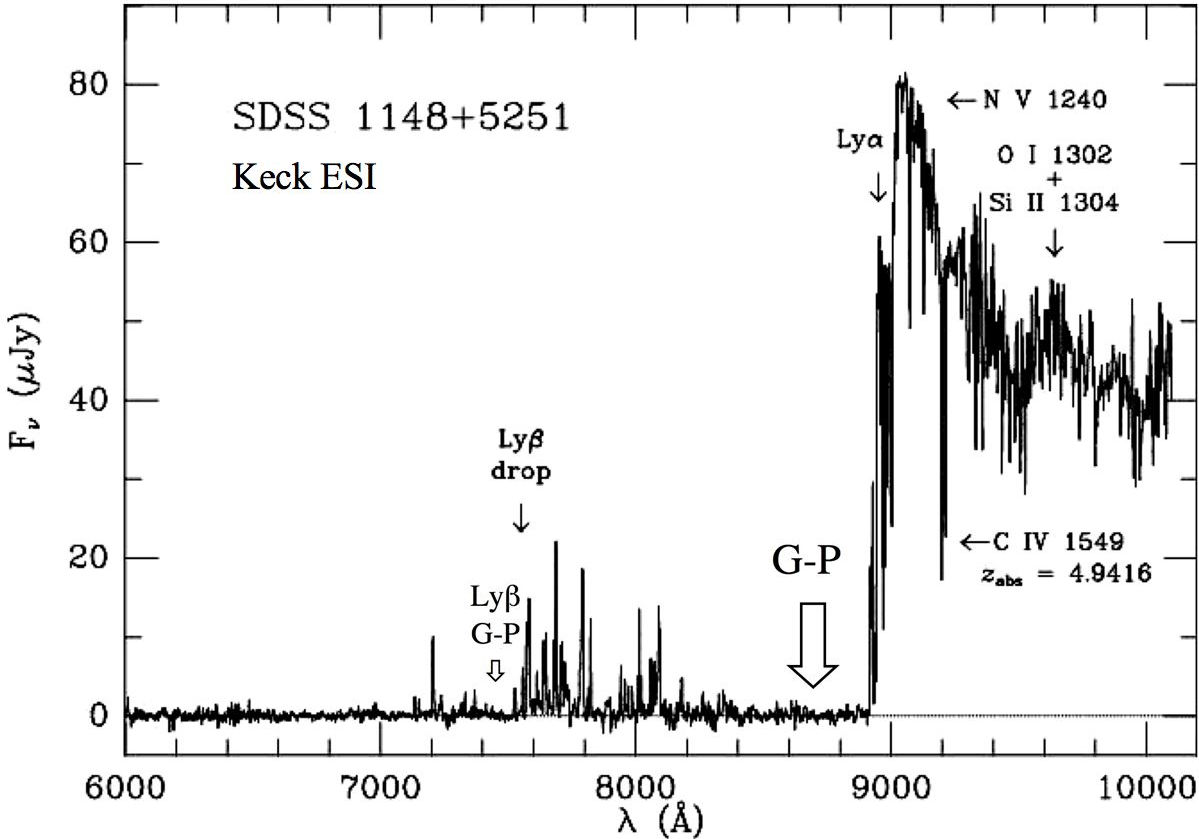
\includegraphics[scale=0.3]{images/dropout.jpg}
\caption{Gunn-Peterson trough in the spectrum of a galaxy at z=6.4.}\label{fig:dropout}
\end{center}		\end{figure}

The spectral flux from distant galaxies redward of the Lyman break is unaffected by Gunn Peterson scattering and remains representative of the true brightness of the luminous object, while the region of the spectrum blueward of the break is highly obscured by the scattering effect of neutral Hydrogen. While the portion of the true emitted spectrum in this region is lost, the extent of the loss contains infomation regarding the optical depth of the intervening space and, thereby, the density of neutral hydrogen at the redshift at which the lyman break falls on that wavelength. Moreover, because the Lyman alpha line invariably falls at a specific point in the emitted spectrum, the redshift of any observed spectrum with an identifiable Lyman break can be measured easily. The break is such a strong spectral feature that it can be located even using broad band photometry, which is a significant advantage for objects at distances such that very little of their emitted light reaches us.\\

\subsection{The Lyman-$\alpha$ Forest}	%%%%%%%%%%%%%%%%%%%%%%%%%%%%%%%

The neutral Hydrogen distribution during cosmic reionization was not homogenous, with expanding bubbles of ionised IGM during the start of ionization and diminishing areas of neutral hydrogen after the central phase of rapid ionization. Regions of the IGM which are relatively underdense in neutral Hydrogen have a correspondingly smaller optical depth to Lyman-$\alpha$ photons passing through them, resulting in sets of peaks on the blueward side of the Lyman break known as the Lyman-$\alpha$ forest. \\

The Lyman forest peaks in figure~\ref{fig:dropout} are typical of galaxies at $z>5$ but the intesity fluctuations in the Lyman forest are largest in regions where the neutral Hydrogen fraction is close to the critical value of $~10^{-5}$, such that even small fluctionations in ionised fraction lead to a large variation in transmitted intensity. An example of this is shown in figure~\ref{fig:forest}.\\
\begin{figure}[h]	\begin{center}
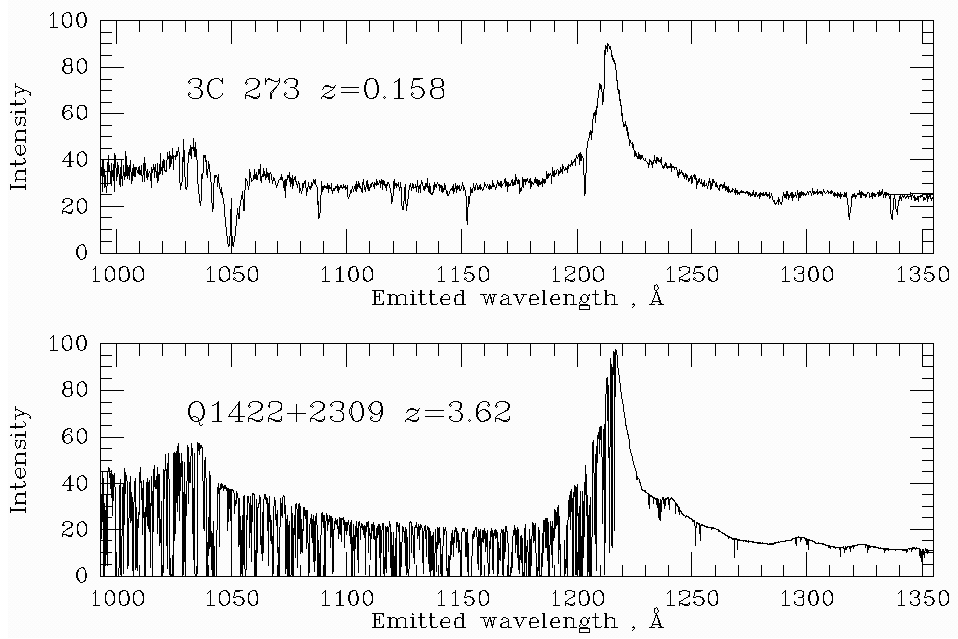
\includegraphics[scale=0.35]{images/forest.png}
\caption{The spectra of two similar galaxies. Above: the spectrum of a galaxy at z=0.158 showing no significant extinction from Gunn Peterson scattering. Below: the spectrum of a galaxy at z=3.62 showing a Lyman forest caused by fluctuations in Hydrogen neutral fraction.}
\label{fig:forest}
\end{center}		\end{figure}

It paradoxically seems, therefore, that the loss of flux caused by the Gunn-Peterson effect is extremely fortuitous to the observational cosmologist. Since the true emitted spectra of Lyman break galaxies are similar in nature to the spectra of closer galaxies with negligible Gunn Peterson absorption, it is theoretically possible, through comparison of observed spectra with models of emitted spectra, to probe the density of neutral Hydrogen at every point between the observed galaxy and the end of reionization.\\

\subsection{Properties of the Lyman-$\alpha$ line}


The full relativistic equation for the energy levels of neutral Hydrogen was calculated by Dirac to be:
\begin{align}
			E_{n,j} = - \frac{e^4}{ (4 \pi \epsilon_0)^2 2 \hbar^2 n^2} \left( \frac{m_p m_e}{m_p + m_e} \right) % E + R, p286
					\left [ 1 + \frac{\alpha^2}{n} \left( \frac{1}{j+1/2} - \frac{3}{4n} \right) \right]
\end{align}

Where $\alpha$ is the fine structure constant:
\begin{align}		
			\alpha = \frac{e^2}{4 \pi \epsilon_0 \hbar c}  \approx \frac{1}{137}.
\end{align}

However, the final factor in square brackets is a small fractional correction of the order $10^{-5}$ or below and replacing the electron-proton reduced mass simply with the electron mass makes a fractional difference of the order of only $10^{-4}$. If we apply both these approximations the equation reduces to the more familiar relation for Hydrogen energy levels which can be derived from the Bohr model of quantum mechanics:

\begin{align}
			E_n = - \frac{m_e e^4}{8 \epsilon_0^2 h^2 n^2}.
\end{align}

Using this result, we can calculate the energy transfer of the n=2 to n=1 transition:

\begin{align}
			\Delta E_{2,1} = E_2 - E_1 = 10.199\; \textup{eV} ,
\end{align}
corresponding to a wavelength of:
\begin{align}
			\lambda_{Ly\alpha} = \frac{hc}{\Delta E_{2,1}} = 1215.7 \; \textup{\AA}.
\end{align}

This means the absorbed photons will invariably be ultraviolet in the absorber rest frame, but for objects observed during the epoch of reionization, cosmological redshift will push the observed Lyman break into the near infrared in the observer frame. The challenges of observing these wavelengths from such large distances and potential methods of overcoming them comprise a large portion of this report. 

%%%% transition diagram

%%%% resonance graph

%%%% fan picture of the troughs

\section{ Galaxy Number Predictions}	%%%%%%%%%%%%%%%%%%%%%%%%%%%%%%%%%%

One of the central tasks of the predictions subgroup is to make informed predictions regarding the distribution of galaxies around and during the epoch of reionization. As previously described, the distribution of galaxies in the early universe can be modelled using a Schechter function:

\begin{align}	
			\Phi_L = \Phi^*  \left(\frac{L}{L^*}\right)^\alpha \exp{\left( -\frac{L}{L^*} \right)} \frac{1}{L^*}
\end{align}

Ultimately, it will be necessary to resort to numerical calculations to extract meaningful predictions from this model, but it is useful and instructive to begin with an analytical approach.

\subsection{Analytical Approach}	%%%%%%%%%%%%%%%%%%%%%%%%%%%%%%%%%%

We use the Schechter function to decribe the number density of galaxies per unit luminosity; in order to extract a true number density from this we must integrate across the relevant range of luminosities:

\begin{align}	
			n = \int_{L_1}^{L_2}  { \Phi_L \; dL } .		
\end{align}

In general, the luminosity function (and, therefore, the number density) will vary as a function of position, $\Phi_L = \Phi_L (L,\underline{\mathbf{r}})$, so in order to extract the number of galaxies in some finite volume we must integrate across the volume

\begin{align}	
			N = \int_V { n(\underline{\mathbf{r}}) \; dV } ,		
\end{align}

resulting in the double integral:

\begin{align}	
			N = \int_V { \int_{L_1}^{L_2}   { \Phi_L(L,\underline{\mathbf{r}})  \; dL } \; dV } .	
\end{align}

If the volume of space considered spans a sufficiently large area of sky then we can invoke the large scale isotropy implied by the cosmological principle to argue that, in effect, $\Phi_L$ is not dependent upon the full position vector, $\underline{\mathbf{r}}$, but only its radial component, $r$. Furthermore, since there is a one to one relationship between distance from earth, $r$, and cosmological redshift, $z$, $\Phi_L$ can be expressed as a function of just $L$ and $z$.

\begin{align}	
			\Phi_L = \Phi_L(L,r);	&&	 r= r(z); 		
\end{align}

\begin{align}
			\therefore	\Phi_L = \Phi_L(L,z).	
\end{align}

The inaccuracy of this simplification on smaller scales is considered in more depth later, in the section on cosmic variance.
The volume of integration can then be chosen to be a spherical shell with limits of constant redshift, so that the volume integration may be carried out over concentric and infinitesimal redshift shells:
\begin{align}
			N = \int_{z_1}^{z_2}  { \int_{L_1}^{L_2} { \Phi_L(L,z) \; dL } \;  \frac{dV}{dz} \; dz }.
\end{align}
From equation !!!comoving integral!!!, we know that:
\begin{align} 
		 	\frac{dr}{dz} &= \frac{c}{H(z)}. 
\end{align}
Together with the form of the volume, we can use this to find the derivative $\frac{dV}{dz}$:
\begin{align}	
					\frac{dV}{dz}  	= \frac{dV}{dr} \cdot \frac{dr}{dz} \;  
 				= \frac{d}{dr} \left[\frac{4}{3} \pi r^3 \right ] \cdot \frac{c}{H(z)} \
				= 4 \pi r^2 \cdot \frac{c}{H(z)} 
\end{align}	
\begin{align}	
			\Rightarrow	\frac{dV}{dz}	= \frac{4 \pi r^2 c}{H(z)}			
\end{align}
Applying this substitution results in 
\begin{align}
			N = \int_{z_1}^{z_2}  { \int_{L_1}^{L_2} { \Phi_L(L,z)  \;  \frac{4 \pi r^2 c}{H(z)} \;  dL \; dz } }
\end{align}

Where the value of r is also found using equation !!!comoving integral!!!

\begin{align}
			N = \int_{z_1}^{z_2}  { \int_{L_1}^{L_2} { \Phi_L(L,z)  \;  \frac{4 \pi c}{H(z)} \;  dL \; dz \left[ \int_0^{z'}{\frac{c }{H(z)} dz'' }\right ]^2} }
\end{align}

In practice, luminosities are most commonly measured in terms of absolute magnitude, M, so in order to align with convention we use the magnitude equivalent of the luminosity function and substitute:

\begin{align}		
			\int { \Phi_L \; dL } = \int { \Phi_M\; dM} ,	
\end{align}

where	

\begin{align}	
			\Phi_M = 0.4 \; \ln(10) \; \Phi^* \; 10^{0.4(M^*-M)(\alpha+1)} \; \exp(-10^{0.4(M^*-M)}) 
\end{align}

to give the result:
\begin{align}	
			N = \int_{z_1}^{z_2}  { \int_{M_1}^{M_2} { \Phi_M(M,z)  \;  \frac{4 \pi c}{H(z)} \;  dM \; dz \left[ \int_0^{z'}{\frac{c }{H(z)} dz'' }\right ]^2} } .
\end{align}

Finally, by substituting in the we substitute in the Schechter function 
\begin{align}
			N = \frac{4 \pi c^3}{H_0^3} \int_{z_1}^{z_2}  \frac{1}{E(z)} \;  \left[ \int_0^{z}{\frac{1}{E(z')} dz' }\right ]^2 dz \int_{M_1}^{M_2} \Phi_M(M,z) \; dM
\end{align}

%%%%%%%%%%%%%%%%%%%%%%%%%%%%%%%%%%

\subsection{Numerical Computation}

The complexity of this analytical solution makes it an impractical approach for real calculations, so in most cases numbers of galaxies are computed numerically by splitting the M and z continuum into a two dimensional array of discrete redshift shells and magnitude bins. The resulting summation takes the form:

\begin{align}
			N = \sum_i \sum_j \; \Phi_M(z_i,M_j) \; \Delta V(z_i) \; \Delta M_j .
\end{align}

Where $\Delta V(z_i)$, is the volume of the thin, but finite spherical shell between redshift $z_i$ and $z_{i+1}$, and is calculated using the standard equation for the volume of a spherical shell:

\begin{align}	
			\Delta V = \frac{4}{3} \; \pi \; ( d_{i+1}^3 - d_{i}^3)
\end{align}

The Schechter parameters used were designed for use with comoving volumes, so the distances used are comoving distances calculated from z using the standard integral relationship given in equation !!!comoving integral!!!, which is also solved numerically. (see part !!!). \\

Equation !!!sum sum!!! can be seen as the direct but approximate equivalent of the double integral:

\begin{align}
			N = \int_V { \int_{M_1}^{M_2}   { \Phi_M(z,M)  \; dM } \; dV } ,
\end{align}

before it is taken to the continuum limit of infinitesimal $\Delta M$ and $\Delta V$, which makes the calculation mathematically exact.

\subsection{Results}	%%%%%%%%%%%%%%%%%%%%%%%%%%%%%

\newpage

\section{Appendices}
%% mostly from 'The Intergalactic Medium' by Piero Madau


\subsection{Derivation of the Gunn-Peterson Optical Depth} \label{appendix:opticaldepth}

The optical depth, $\tau$, of a medium to light of some frequency, $\nu$, can be calculated using:
\begin{align}
			\tau = \sigma(\nu) N ,
\end{align}
where N is the column density, calculated using:
\begin{align}
			N = \int n dl .
\end{align}
Therefore, for the optical depth of neutral Hydrogen in the early universe, we have:
\begin{align}
			\tau = \int{} \sigma ( \nu ) n_{HI}(z) dl    
			        = \int{} \sigma ( \nu ) n_{HI}(z) \frac{dl}{dz} dz
\end{align}
From the proper line element of the Friedman-Robertson-Walker metric the derivative of the proper distance, $l$, can be decuced to be:
\begin{align}
			\frac{dl}{dz} = \frac{c}{(1+z) H(z)} ,
\end{align}
and the scattering cross-section of Hydrogen is:
\begin{align}
			\sigma (\nu) = \frac{\mu_0 e^2 c}{4 m_e} f \phi(\nu)
\end{align}
where f is the upward oscillator strength of the transition, with a value of 0.4162 for the Lyman$\alpha$ transition and $\phi(\nu)$ is the normalised line profile. Since the scattering cross section is highly resonant at the Lyman-$\alpha$ frequency and negligible elsewhere, $\phi$ can be approximated by the form of a delta function $\phi(\nu) = \delta (\nu - \nu_\alpha)$ . \\

The mean density of neutral Hydrogen can be calculated from the baryon density, $\Omega_b$. We start with the definition of $\Omega_b$:
\begin{align}
			\rho_b = \rho_{crit} \; \Omega_b =  \frac{3H_0^2}{ 8 \pi G} \; \Omega_b = \frac{3H_0^2}{ 8 \pi G} \; \Omega_{b0}(1+z)^3,
\end{align}
we then note that the total baryonic density is also equal to the sum of the separate densities of light elements, which is dominated by Hydrogen and Helium:
\begin{align}
			\rho_b = \sum_{elements} \rho_i \; \approx \; \rho_H + \rho_{He} = \rho_H + Y\rho_b,
\end{align}
where Y is the primordial abundance, by mass, of He with a value Y = $0.247 \pm 0.02$. Equating the two resulting expressions for $\rho_b$ gives:
\begin{align}
			 \frac{3H_0^2}{ 8 \pi G} \; \Omega_{b0}(1+z)^3 = \frac{\rho_H}{1-Y} = \frac{n_H m_H}{1-Y}
\end{align}
\begin{align}
			 \Rightarrow \overline{n}_H &= \frac{3  H_0^2 (1-Y)}{ 8 \pi G m_H} \Omega_{b0} (1+z)^3 \\
			 \Rightarrow \overline{n}_H &= \overline{n}_{H0} (1+z)^3 . 
\end{align} 

The average number density of neutral Hydrogen is this quantity scaled by the neutral fraction, $x_{HI}$:
\begin{align}
			 \overline{n}_{HI} = \overline{n}_H x_{HI} = \overline{n}_{H0} \; (1+z)^3 \; x_{HI} . 
\end{align} 

Combining equations tau, differential, sigma and nH gives:

\begin{align}
\tau_{GP} &= \int_0^{z_e} \frac{\mu_0 e^2 c f}{4 m_e} \; \delta(\nu - \nu_\alpha) \; \overline{n}_{H0} \; \frac{ (1+z)^3 c}{(1+z) H(z)} \; x_{HI} dz \\ \\
&= \frac{ \overline{n}_{H0} \; \mu_0 e^2 c^2 f}{4 m_e H_0} \int_0^{z_e} \delta(\nu - \nu_\alpha) \;  \frac{(1+z)^2}{ E(z)} x_{HI} dz 
\end{align}

For high redshift galaxies, we can use the Einstein-de Sitter approximation for the Hubble parameter evolution:
\begin{align}
			E(z) = \sqrt{ \Omega_\Lambda + \Omega_{M0} (1+z)^3 + \Omega_{R0} (1+z)^4} \approx \sqrt{\Omega_{M0}}(1+z)^{3/2}.
\end{align}
We can also calculate the constant prefactor to have a value:
\begin{align}
		\frac{ \overline{n}_{H0} \; \mu_0 e^2 c^2 f}{4 m_e H_0} = (8.621\times 10^{20} ) \; h \; \Omega_{b0}
\end{align}
Therefore:
\begin{align}
\tau_{GP} =   (8.621\times 10^{20} ) \frac{h \Omega_{b0}}{\sqrt{\Omega_{M0}}}  \int_0^{z_e} \delta(\nu - \nu_\alpha) \;  (1+z)^{1/2} \; x_{HI} \; dz
\end{align}

The frequency of observed radiation, $\nu_0$ can be related to the frequency of the same radiation at some redshift, $z$, by:
\begin{align}
			\nu (z) = \nu_0(1+z)  &&
	\Rightarrow 	\frac{d\nu}{dz} = \nu_0.
\end{align}

This allows us to write the integral purely in terms of $\nu$ and the action of the delta function is then to simply pick out the value of the integrand at the point $\nu = \nu_\alpha$. For convenience, we name the integral part $I$:

\begin{align}
			I &=  \int_0^{z_e} \delta(\nu - \nu_\alpha) \;  (1+z)^{1/2} x_{HI}\; dz \\ 
			  &=  \int_{\nu_0}^{\nu_e} \delta(\nu - \nu_\alpha) \;  \sqrt{\frac{\nu}{\nu_0}} \; \frac{dz}{d\nu} \; x_{HI}\; d\nu \\
			  &=  \int_{\nu_0}^{\nu_e} \delta(\nu - \nu_\alpha) \;  \sqrt{\frac{\nu}{\nu_0^3}} \; x_{HI}\; d\nu \\ 
			  &=  \sqrt{\frac{\nu_\alpha}{\nu_0^3}} \; x_{HI} \\
			  &=  \sqrt{ \frac{(1+z)^3}{\nu_\alpha^2}}\; x_{HI} \\
	\Rightarrow	I &=  \frac{(1+z)^{3/2}}{\nu_\alpha}\; x_{HI}
\end{align}
Note that if $\nu_\alpha$ does not fall within the limits of integration then both the integral and the resulting optical depth is zero. This is the case for the flux which falls on the redward side of the Lyman break. \\

Substituting the new value for the integral back into the optical depth equations gives:
\begin{align}
			\tau_{GP} &=  \frac{(8.621\times 10^{20} )}{\nu_\alpha} \frac{h \Omega_{b0}}{\sqrt{\Omega_{M0}}} \; (1+z)^{3/2} \; x_{HI} \\
				       &=  (3.494 \times 10^{5}) \frac{h \Omega_{b0}}{\sqrt{\Omega_{M0}}} \; (1+z)^{3/2} \; x_{HI}.
\end{align}

This is conventionally writen in the form:
\begin{align}
			\tau_{GP} = 3.59 \times 10^5 \; 	\left ( 	\frac{\Omega_m h^2}{0.13}	\right ) ^{-1/2}	
								\left ( 	\frac{\Omega_b h^2}{0.02}	\right ) 	
								\left ( 	\frac{1+z}{7}			\right )^{3/2} 	
								\left ( 	\frac{n_{HI}}{n_H}			\right ) .
\end{align}

\newpage

\subsection{Derivation of Magnitude Schechter function}

The luminosity function of galaxies is the object, $\Phi_L$, such that the number density of galaxies can be calculated as:
\begin{align}		
			n = \int { \Phi_L \; dL }.\label{eq:nfromphiL}
\end{align}
We, therefore define the magnitude equivalent of the luminosity function to be the object, $\Phi_M$, which obeys the equivalent formula:
\begin{align}		
			n = \int { \Phi_M \; dM }.\label{eq:nfromphiM}.
\end{align}
From equation~\ref{eq:nfromphiL}, we deduce that:
\begin{align}		
			n = \int { \Phi_L \; \frac{dL}{dM}\; dM },
\end{align}
it is then clear, from comparison of this result with equation~\ref{eq:nfromphiM}, that:
\begin{align}		
			\Phi_M = \Phi_L \; \frac{dL}{dM}.\label{eq:conversion}.
\end{align}
We then choose the standard Schechter function as our model of the luminosity function and aim to derive the form of it's magnitude equivalent, $\Phi_M(M)$.
\begin{align}	
			\Phi_L = \Phi^*  \left(\frac{L}{L^*}\right)^\alpha \exp{\left( -\frac{L}{L^*} \right)} \frac{1}{L^*}
\end{align}

\begin{align}	
			M &= -2.5\log_{10}\left ( \frac{L}{L_0}\right) \\
			   &= \frac{-2.5}{\ln(10)} \ln\left ( \frac{L}{L_0}\right) \\ \\
	\Rightarrow \frac{dM}{dL} &= \frac{-2.5}{\ln(10)} \frac{1}{L}
\end{align}
Substituting this result into equation~\ref{eq:conversion}, gives:
\begin{align}		
			\Phi_M(L) &= \frac{-L\ln(10)}{2.5} \Phi^*  \left(\frac{L}{L^*}\right)^\alpha \exp{\left( \frac{-L}{L^*} \right)} \frac{1}{L^*} \\
				     &= \frac{-\ln(10)}{2.5} \Phi^*  \left(\frac{L}{L^*}\right)^{\alpha+1} \exp{\left( \frac{-L}{L^*} \right)} 
\end{align}
\begin{align}
			M - M^* = -2.5 \log_{10}\left( \frac{L}{L^*} \right)	\\
			\left( \frac{L}{L^*} \right)	 = 10^{0.4(M^*-M)}
\end{align}
Finally, we apply this substitution:
\begin{align}		
			\Phi_M(M) = \frac{-\ln(10)}{2.5} \Phi^*  10^{0.4(M^*-M)(\alpha+1)} \exp(-10^{0.4(M^*-M)}) .
\end{align}
In practice, the minus sign is accounted for by inverting the limits of integration and integrating from low M to high M (dim galaxies to bright galaxies).

\newpage

\subsection{Derivation of Light travel Distance}

\begin{align}
			dl = cdt.
\end{align}
If there is a 1:1 relationship between scale factor, a, and time, t, then we can say 
\begin{align}
			dt = \frac{dt}{da} \; da = \frac{da}{\dot{a}}
\end{align}
We then use:
\begin{align}
			 a = \frac{1}{1+z} 
\end{align}
\begin{align}
	\Rightarrow da = -\frac{dz}{(1+z)^2} = -\frac{dz \; a}{1+z}.
\end{align}
and by the definition of the Hubble parameter, $H(z) = \frac{\dot{a}}{a}$, so:
\begin{align}
			dt = \frac{da}{\dot{a}} = \frac{-dz }{1+z} \; \frac{a}{\dot{a}} = \frac {-dz}{(1+z) H(z)}
\end{align}
\begin{align}
			l = \int c \; dt = \int_z^0 \frac {-dz'}{(1+z') H(z')}
\end{align}

\begin{align}
		\Rightarrow l = \int_0^z \frac {dz'}{(1+z') H(z')}
\end{align}

% schechter z dependence is implicit in parameters
% graphs
% luminosity functions with z
% parameters with z
% m with z
% DV with z

% convergance!

%%%%%%%%%%%%%%%%%%%%%%%%%%%%%%%%%%%%%%%


\end{document}
